\section{Fundamentação Teórica}
\subsection{Definição de Teoria dos Jogos}
\begin{frame}
\frametitle{Definição de Teoria dos Jogos}
\begin{block}{}
	A \textbf{Teoria dos Jogos} é uma área de estudos derivada da matemática que estuda o comportamento de indivíduos sob uma situação de conflito.
\end{block}
\begin{itemize}
	\item Teoria Econômica dos Jogos
	\item Teoria Combinatória dos Jogos
	\item Teoria Computacional dos Jogos
\end{itemize}
\end{frame}

\subsubsection{Teoria Econômica dos Jogos}
\begin{frame}
\frametitle{\subsubsecname}
\begin{itemize}
	\item[1921] Émile Borel, reinventou Minimax
	\item[1944] von Neumann and Morgenstern
	\item Jogo de Soma Zero
	\item Jogo Cooperativo e Não Cooperativo
	\item[1950] John Forbes Nash
	\item Equilíbrio de Nash (Estratégias Mistas)
\end{itemize}
\end{frame}

\begin{frame}[fragile]
\frametitle{Representação}
\begin{lstlisting}
    Game = <Jogadores, Strategy, Payoffs>
\end{lstlisting}
\pause
\begin{equation*}
\begin{split}
  J\ &=\ \{j_1, j_2,...,j_i\}\\
  \pause
  S_{i}\ &=\ \{s_{i1},s_{i2},...,s_{ij}\},\\
  \pause
  \forall j_i\!\in\!J&,\ \exists\ s_{ij}\!\in\!S_i\\
  \pause
  P_i &: S_{i}\rightarrow\mathbb{R}
\end{split}
\end{equation*}
\end{frame}

\subsubsection{Teoria Combinatória dos Jogos}
\begin{frame}[fragile]
\frametitle{\subsubsecname}
\begin{equation*}
\begin{split}
  G\ &=\ \{G^L|G^R\}, \text{Representação de jogo}\\
  \pause
  \{\emptyset|\emptyset\}\ &=\ \{|\}, \text{Fim de jogo}\\
  \pause
  *\ &=\ \{0|0\}, \text{Estrela, próximo jogador ganha}\\
  \pause
  \uparrow\ &=\ \{0|*\}, \text{Left sempre ganha}\\
  \pause
  \downarrow\ &=\ \{*|0\}, \text{Right sempre ganha}\\
\end{split}
\end{equation*}
\end{frame}

\subsubsection{Teoria Computacional dos Jogos}
\begin{frame}[fragile]
\frametitle{\subsubsecname}
Engloba jogos que podem ser resolvidos por força bruta ou que podem ser jogados contra uma Inteligência Artificial.
\begin{itemize}
	\item Para jogos pequenos é possível percorrer todas as possibilidades
	\item Para jogos maiores, é necessário uma função que avalie a posição atual
\end{itemize}
\end{frame}

\begin{frame}[fragile]
\frametitle{\subsubsecname}
Dois jogadores alternam turnos. O estado do nó indica a situação do jogador da vez. Estados possíveis na árvore:
\begin{itemize}
	\item[\textcolor{green}{\textbullet}] \emph{Vencedor} ($\exists$ um nó filho \emph{Perdedor})
	\item[\textcolor{red}{\textbullet}] \emph{Perdedor} (Todos os nós filho são \emph{Vencedores})
	\item[\textcolor{yellow}{\textbullet}] Empate ($\nexists$ nó filho \emph{Perdedor}, $\exists$ nó filho \emph{Empate})
\end{itemize}
\end{frame}

\subsection{Representação e Soluções de Jogos}
\begin{frame}
\frametitle{\secname}
Há duas maneiras de representar um jogo:
\begin{itemize}
	\item Forma Extensa
	\item Forma Normal (Matriz de \emph{payoff})
\end{itemize}
\end{frame}

\subsubsection*{Renée v Peter}
\begin{frame}
\frametitle{\subsecname}
\begin{itemize}
	\item Dois jogadores: \textbf{\emph{Renée}} e \textbf{\emph{Peter}}
	\pause
	\item Três cartas: Rei (\textbf{\emph{K}}), Dez (\textbf{\emph{T}}) e Dois (\textbf{\emph{D}})
	\pause
	\item[\emph{R}] Escolhe uma carta
	\pause
	\item[\emph{P}] Adivinha se \emph{\textbf{Alta}} (\emph{K}) ou \emph{\textbf{Baixa}} (\emph{D})
	\pause
	\begin{itemize}
		\item[\emph{P}] erra, \emph{R} ganha 2
		\pause
		\item[\emph{P}] acerta, \emph{R} perde 3
	\end{itemize}
	\pause
	\item No caso $T$
	\pause
	\begin{itemize}
		\item[\emph{Baixa}] \emph{R} ganha 1
		\pause
		\item[\emph{Alta}] \emph{R} escolhe outra carta
	\end{itemize}
	\pause
	\begin{itemize}
		\item[\emph{P}] erra, \emph{R} ganha 3
		\pause
		\item[\emph{P}] acerta, \emph{R} perde 1
	\end{itemize}
\end{itemize}
\end{frame}

\subsubsection*{Forma Extensa}
\begin{frame}
\frametitle{Forma Extensa\\Vez de \emph{Renée}}
\begin{figure}[ht]
	\centering
	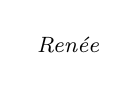
\begin{tikzpicture}
	  [
	    grow                    = down,
	    edge from parent/.style = {draw, -latex},
	    every node/.style       = {font=\footnotesize},
	    sloped,
		level 1/.style			= {
			sibling distance=2.5cm,
			level distance=1cm
		},
		level 2/.style			= {
			sibling distance=1.5cm,
			level distance=1.5cm
		},
		level 3/.style			= {
			sibling distance=2cm,
			level distance=1cm
		},
		level 4/.style			= {
			sibling distance=1.5cm,
			level distance=1.5cm
		}
		]
		\node {\emph{Renée}};
	\end{tikzpicture}
\end{figure}
\end{frame}

\begin{frame}
\frametitle{Forma Extensa\\Opções de \emph{Renée}}
\begin{figure}[ht]
	\centering
	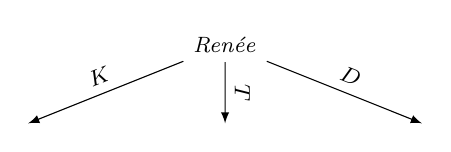
\begin{tikzpicture}
	  [
	    grow                    = down,
	    edge from parent/.style = {draw, -latex},
	    every node/.style       = {font=\footnotesize},
	    sloped,
		level 1/.style			= {
			sibling distance=2.5cm,
			level distance=1cm
		},
		level 2/.style			= {
			sibling distance=1.5cm,
			level distance=1.5cm
		},
		level 3/.style			= {
			sibling distance=2cm,
			level distance=1cm
		},
		level 4/.style			= {
			sibling distance=1.5cm,
			level distance=1.5cm
		}
		]
		\node {\emph{Renée}}
		child {
			edge from parent node [above] {$K$}
		}
		child {
			edge from parent node [above] {$T$}
		}
		child {
			edge from parent node [above] {$D$}
		};
	\end{tikzpicture}
\end{figure}
\end{frame}

\begin{frame}
\frametitle{Forma Extensa\\Vez de \emph{Peter}}
\begin{figure}[ht]
	\centering
	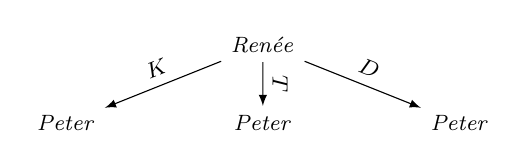
\begin{tikzpicture}
	  [
	    grow                    = down,
	    edge from parent/.style = {draw, -latex},
	    every node/.style       = {font=\footnotesize},
	    sloped,
		level 1/.style			= {
			sibling distance=2.5cm,
			level distance=1cm
		},
		level 2/.style			= {
			sibling distance=1.5cm,
			level distance=1.5cm
		},
		level 3/.style			= {
			sibling distance=2cm,
			level distance=1cm
		},
		level 4/.style			= {
			sibling distance=1.5cm,
			level distance=1.5cm
		}
		]
		\node {\emph{Renée}}
		child {
			node (P1){\emph{Peter}} {
			}
			edge from parent node [above] {$K$}
		}
		child {
			node (P2) {\emph{Peter}} {
			}
			edge from parent node [above] {$T$}
		}
		child {
			node (P3) {\emph{Peter}} {
			}
			edge from parent node [above] {$D$}
		};
	\end{tikzpicture}
\end{figure}
\end{frame}

\begin{frame}
\frametitle{Forma Extensa\\Conjunto de Informação}
\begin{figure}[ht]
	\centering
	\begin{tikzpicture}
	  [
	    grow                    = down,
	    edge from parent/.style = {draw, -latex},
	    every node/.style       = {font=\footnotesize},
	    sloped,
		level 1/.style			= {
			sibling distance=2.5cm,
			level distance=1cm
		},
		level 2/.style			= {
			sibling distance=1.5cm,
			level distance=1.5cm
		},
		level 3/.style			= {
			sibling distance=2cm,
			level distance=1cm
		},
		level 4/.style			= {
			sibling distance=1.5cm,
			level distance=1.5cm
		}
		]
		\node {\emph{Renée}}
		child {
			node (P1){\emph{Peter}} {
			}
			edge from parent node [above] {$K$}
		}
		child {
			node (P2) {\emph{Peter}} {
			}
			edge from parent node [above] {$T$}
		}
		child {
			node (P3) {\emph{Peter}} {
			}
			edge from parent node [above] {$D$}
		};
		\draw[thick, rounded corners] ($(P1.north west)+(-0.1,-0.1)$) rectangle ($(P3.south east)+(0.1,+0.1)$);
	\end{tikzpicture}
\end{figure}
\end{frame}

\begin{frame}
\frametitle{Forma Extensa\\Opções de \emph{Peter}}
\begin{figure}[ht]
	\centering
	\begin{tikzpicture}
	  [
	    grow                    = down,
	    edge from parent/.style = {draw, -latex},
	    every node/.style       = {font=\footnotesize},
	    sloped,
		level 1/.style			= {
			sibling distance=2.5cm,
			level distance=1cm
		},
		level 2/.style			= {
			sibling distance=1.5cm,
			level distance=1.5cm
		},
		level 3/.style			= {
			sibling distance=2cm,
			level distance=1cm
		},
		level 4/.style			= {
			sibling distance=1.5cm,
			level distance=1.5cm
		}
		]
		\node {\emph{Renée}}
		child {
			node (P1){\emph{Peter}} {
				child {
					node {}
				}
				child {
					node {}
				}
			}
			edge from parent node [above] {$K$}
		}
		child {
			node (P2) {\emph{Peter}} {
				child {
					node (R) {}{
					}
				}
				child {
				node {}
				}
			}
			edge from parent node [above] {$T$}
		}
		child {
			node (P3) {\emph{Peter}} {
				child {
					node {}
				}
				child {
					node {}
				}
			}
			edge from parent node [above] {$D$}
		};
		\draw[thick, rounded corners] ($(P1.north west)+(-0.1,-0.1)$) rectangle ($(P3.south east)+(0.1,+0.1)$);
	\end{tikzpicture}
\end{figure}
\end{frame}

\begin{frame}
\frametitle{Forma Extensa\\Opções de \emph{Peter}}
\begin{figure}[ht]
	\centering
	\begin{tikzpicture}
	  [
	    grow                    = down,
	    edge from parent/.style = {draw, -latex},
	    every node/.style       = {font=\footnotesize},
	    sloped,
		level 1/.style			= {
			sibling distance=2.5cm,
			level distance=1cm
		},
		level 2/.style			= {
			sibling distance=1.5cm,
			level distance=1.5cm
		},
		level 3/.style			= {
			sibling distance=2cm,
			level distance=1cm
		},
		level 4/.style			= {
			sibling distance=1.5cm,
			level distance=1.5cm
		}
		]
		\node {\emph{Renée}}
		child {
			node (P1){\emph{Peter}} {
				child {
					node {}
					edge from parent node [above] {\emph{Alta}}
				}
				child {
					node {}
				}
			}
			edge from parent node [above] {$K$}
		}
		child {
			node (P2) {\emph{Peter}} {
				child {
					node (R) {}{
					}
					edge from parent node [above] {\emph{Alta}}
				}
				child {
				node {}
				}
			}
			edge from parent node [above] {$T$}
		}
		child {
			node (P3) {\emph{Peter}} {
				child {
					node {}
					edge from parent node [above] {\emph{Alta}}
				}
				child {
					node {}
				}
			}
			edge from parent node [above] {$D$}
		};
		\draw[thick, rounded corners] ($(P1.north west)+(-0.1,-0.1)$) rectangle ($(P3.south east)+(0.1,+0.1)$);
	\end{tikzpicture}
\end{figure}
\end{frame}

\begin{frame}
\frametitle{Forma Extensa\\Opções de \emph{Peter}}
\begin{figure}[ht]
	\centering
	\begin{tikzpicture}
	  [
	    grow                    = down,
	    edge from parent/.style = {draw, -latex},
	    every node/.style       = {font=\footnotesize},
	    sloped,
		level 1/.style			= {
			sibling distance=2.5cm,
			level distance=1cm
		},
		level 2/.style			= {
			sibling distance=1.5cm,
			level distance=1.5cm
		},
		level 3/.style			= {
			sibling distance=2cm,
			level distance=1cm
		},
		level 4/.style			= {
			sibling distance=1.5cm,
			level distance=1.5cm
		}
		]
		\node {\emph{Renée}}
		child {
			node (P1){\emph{Peter}} {
				child {
					node {}
					edge from parent node [above] {\emph{Alta}}
				}
				child {
					node {}
					edge from parent node [above] {\emph{Baixa}}
				}
			}
			edge from parent node [above] {$K$}
		}
		child {
			node (P2) {\emph{Peter}} {
				child {
					node (R) {}{
					}
					edge from parent node [above] {\emph{Alta}}
				}
				child {
				node {}
				edge from parent node [above] {\emph{Baixa}}
				}
			}
			edge from parent node [above] {$T$}
		}
		child {
			node (P3) {\emph{Peter}} {
				child {
					node {}
					edge from parent node [above] {\emph{Alta}}
				}
				child {
					node {}
					edge from parent node [above] {\emph{Baixa}}
				}
			}
			edge from parent node [above] {$D$}
		};
		\draw[thick, rounded corners] ($(P1.north west)+(-0.1,-0.1)$) rectangle ($(P3.south east)+(0.1,+0.1)$);
	\end{tikzpicture}
\end{figure}
\end{frame}

\begin{frame}
\frametitle{Forma Extensa\\Se \emph{Peter} errar}
\begin{figure}[ht]
	\centering
	\begin{tikzpicture}
	  [
	    grow                    = down,
	    edge from parent/.style = {draw, -latex},
	    every node/.style       = {font=\footnotesize},
	    sloped,
		level 1/.style			= {
			sibling distance=2.5cm,
			level distance=1cm
		},
		level 2/.style			= {
			sibling distance=1.5cm,
			level distance=1.5cm
		},
		level 3/.style			= {
			sibling distance=2cm,
			level distance=1cm
		},
		level 4/.style			= {
			sibling distance=1.5cm,
			level distance=1.5cm
		}
		]
		\node {\emph{Renée}}
		child {
			node (P1){\emph{Peter}} {
				child {
					node {}
					edge from parent node [above] {\emph{Alta}}
				}
				child {
					node {\textbf{2}}
					edge from parent node [above] {\emph{Baixa}}
				}
			}
			edge from parent node [above] {$K$}
		}
		child {
			node (P2) {\emph{Peter}} {
				child {
					node (R) {}{
					}
					edge from parent node [above] {\emph{Alta}}
				}
				child {
				node {}%{\textbf{1}}
				edge from parent node [above] {\emph{Baixa}}
				}
			}
			edge from parent node [above] {$T$}
		}
		child {
			node (P3) {\emph{Peter}} {
				child {
					node {\textbf{2}}
					edge from parent node [above] {\emph{Alta}}
				}
				child {
					node {}
					edge from parent node [above] {\emph{Baixa}}
				}
			}
			edge from parent node [above] {$D$}
		};
		\draw[thick, rounded corners] ($(P1.north west)+(-0.1,-0.1)$) rectangle ($(P3.south east)+(0.1,+0.1)$);
	\end{tikzpicture}
\end{figure}
\end{frame}

\begin{frame}
\frametitle{Forma Extensa\\Se \emph{Peter} acertar}
\begin{figure}[ht]
	\centering
	\begin{tikzpicture}
	  [
	    grow                    = down,
	    edge from parent/.style = {draw, -latex},
	    every node/.style       = {font=\footnotesize},
	    sloped,
		level 1/.style			= {
			sibling distance=2.5cm,
			level distance=1cm
		},
		level 2/.style			= {
			sibling distance=1.5cm,
			level distance=1.5cm
		},
		level 3/.style			= {
			sibling distance=2cm,
			level distance=1cm
		},
		level 4/.style			= {
			sibling distance=1.5cm,
			level distance=1.5cm
		}
		]
		\node {\emph{Renée}}
		child {
			node (P1){\emph{Peter}} {
				child {
					node {\textbf{-3}}
					edge from parent node [above] {\emph{Alta}}
				}
				child {
					node {\textbf{2}}
					edge from parent node [above] {\emph{Baixa}}
				}
			}
			edge from parent node [above] {$K$}
		}
		child {
			node (P2) {\emph{Peter}} {
				child {
					node (R) {}{
					}
					edge from parent node [above] {\emph{Alta}}
				}
				child {
				node {}
				edge from parent node [above] {\emph{Baixa}}
				}
			}
			edge from parent node [above] {$T$}
		}
		child {
			node (P3) {\emph{Peter}} {
				child {
					node {\textbf{2}}
					edge from parent node [above] {\emph{Alta}}
				}
				child {
					node {\textbf{-3}}
					edge from parent node [above] {\emph{Baixa}}
				}
			}
			edge from parent node [above] {$D$}
		};
		\draw[thick, rounded corners] ($(P1.north west)+(-0.1,-0.1)$) rectangle ($(P3.south east)+(0.1,+0.1)$);
	\end{tikzpicture}
\end{figure}
\end{frame}


\begin{frame}
\frametitle{Forma Extensa\\Caso \emph{T}}
\begin{figure}[ht]
	\centering
	\begin{tikzpicture}
	  [
	    grow                    = down,
	    edge from parent/.style = {draw, -latex},
	    every node/.style       = {font=\footnotesize},
	    sloped,
		level 1/.style			= {
			sibling distance=2.5cm,
			level distance=1cm
		},
		level 2/.style			= {
			sibling distance=1.5cm,
			level distance=1.5cm
		},
		level 3/.style			= {
			sibling distance=2cm,
			level distance=1cm
		},
		level 4/.style			= {
			sibling distance=1.5cm,
			level distance=1.5cm
		}
		]
		\node {\emph{Renée}}
		child {
			node (P1){\emph{Peter}} {
				child {
					node {\textbf{-3}}
					edge from parent node [above] {\emph{Alta}}
				}
				child {
					node {\textbf{2}}
					edge from parent node [above] {\emph{Baixa}}
				}
			}
			edge from parent node [above] {$K$}
		}
		child {
			node (P2) {\emph{Peter}} {
				child {
					node (R) {}{
					}
					edge from parent node [above] {\emph{Alta}}
				}
				child {
				node {\textbf{1}}
				edge from parent node [above] {\emph{Baixa}}
				}
			}
			edge from parent node [above] {$T$}
		}
		child {
			node (P3) {\emph{Peter}} {
				child {
					node {\textbf{2}}
					edge from parent node [above] {\emph{Alta}}
				}
				child {
					node {\textbf{-3}}
					edge from parent node [above] {\emph{Baixa}}
				}
			}
			edge from parent node [above] {$D$}
		};
		\draw[thick, rounded corners] ($(P1.north west)+(-0.1,-0.1)$) rectangle ($(P3.south east)+(0.1,+0.1)$);
	\end{tikzpicture}
\end{figure}
\end{frame}


\begin{frame}
\frametitle{Forma Extensa\\Vez de \emph{Renée}}
\begin{figure}[ht]
	\centering
	\begin{tikzpicture}
	  [
	    grow                    = down,
	    edge from parent/.style = {draw, -latex},
	    every node/.style       = {font=\footnotesize},
	    sloped,
		level 1/.style			= {
			sibling distance=2.5cm,
			level distance=1cm
		},
		level 2/.style			= {
			sibling distance=1.5cm,
			level distance=1.5cm
		},
		level 3/.style			= {
			sibling distance=2cm,
			level distance=1cm
		},
		level 4/.style			= {
			sibling distance=1.5cm,
			level distance=1.5cm
		}
		]
		\node {\emph{Renée}}
		child {
			node (P1){\emph{Peter}} {
				child {
					node {\textbf{-3}}
					edge from parent node [above] {\emph{Alta}}
				}
				child {
					node {\textbf{2}}
					edge from parent node [above] {\emph{Baixa}}
				}
			}
			edge from parent node [above] {$K$}
		}
		child {
			node (P2) {\emph{Peter}} {
				child {
					node (R) {\emph{Renée}} {
					}
					edge from parent node [above] {\emph{Alta}}
				}
				child {
				node {\textbf{1}}
				edge from parent node [above] {\emph{Baixa}}
				}
			}
			edge from parent node [above] {$T$}
		}
		child {
			node (P3) {\emph{Peter}} {
				child {
					node {\textbf{2}}
					edge from parent node [above] {\emph{Alta}}
				}
				child {
					node {\textbf{-3}}
					edge from parent node [above] {\emph{Baixa}}
				}
			}
			edge from parent node [above] {$D$}
		};
		\draw[thick, rounded corners] ($(P1.north west)+(-0.1,-0.1)$) rectangle ($(P3.south east)+(0.1,+0.1)$);
	\end{tikzpicture}
\end{figure}
\end{frame}

\begin{frame}
\frametitle{Forma Extensa\\Opções de \emph{Renée}}
\begin{figure}[ht]
	\centering
	\begin{tikzpicture}
	  [
	    grow                    = down,
	    edge from parent/.style = {draw, -latex},
	    every node/.style       = {font=\footnotesize},
	    sloped,
		level 1/.style			= {
			sibling distance=2.5cm,
			level distance=1cm
		},
		level 2/.style			= {
			sibling distance=1.5cm,
			level distance=1.5cm
		},
		level 3/.style			= {
			sibling distance=2cm,
			level distance=1cm
		},
		level 4/.style			= {
			sibling distance=1.5cm,
			level distance=1.5cm
		}
		]
		\node {\emph{Renée}}
		child {
			node (P1){\emph{Peter}} {
				child {
					node {\textbf{-3}}
					edge from parent node [above] {\emph{Alta}}
				}
				child {
					node {\textbf{2}}
					edge from parent node [above] {\emph{Baixa}}
				}
			}
			edge from parent node [above] {$K$}
		}
		child {
			node (P2) {\emph{Peter}} {
				child {
					node (R) {\emph{Renée}} {
						child {
							edge from parent node [above] {$K$}
						}
						child {
							edge from parent node [above] {$D$}
						}
					}
					edge from parent node [above] {\emph{Alta}}
				}
				child {
				node {\textbf{1}}
				edge from parent node [above] {\emph{Baixa}}
				}
			}
			edge from parent node [above] {$T$}
		}
		child {
			node (P3) {\emph{Peter}} {
				child {
					node {\textbf{2}}
					edge from parent node [above] {\emph{Alta}}
				}
				child {
					node {\textbf{-3}}
					edge from parent node [above] {\emph{Baixa}}
				}
			}
			edge from parent node [above] {$D$}
		};
		\draw[thick, rounded corners] ($(P1.north west)+(-0.1,-0.1)$) rectangle ($(P3.south east)+(0.1,+0.1)$);
	\end{tikzpicture}
\end{figure}
\end{frame}

\begin{frame}
\frametitle{Forma Extensa\\Vez de \emph{Peter}}
\begin{figure}[ht]
	\centering
	\begin{tikzpicture}
	  [
	    grow                    = down,
	    edge from parent/.style = {draw, -latex},
	    every node/.style       = {font=\footnotesize},
	    sloped,
		level 1/.style			= {
			sibling distance=2.5cm,
			level distance=1cm
		},
		level 2/.style			= {
			sibling distance=1.5cm,
			level distance=1.5cm
		},
		level 3/.style			= {
			sibling distance=2cm,
			level distance=1cm
		},
		level 4/.style			= {
			sibling distance=1.5cm,
			level distance=1.5cm
		}
		]
		\node {\emph{Renée}}
		child {
			node (P1){\emph{Peter}} {
				child {
					node {\textbf{-3}}
					edge from parent node [above] {\emph{Alta}}
				}
				child {
					node {\textbf{2}}
					edge from parent node [above] {\emph{Baixa}}
				}
			}
			edge from parent node [above] {$K$}
		}
		child {
			node (P2) {\emph{Peter}} {
				child {
					node (R) {\emph{Renée}} {
						child {
							node (P21) {\emph{Peter}} {
							}
							edge from parent node [above] {$K$}
						}
						child {
							node (P22) {\emph{Peter}} {
							}
							edge from parent node [above] {$D$}
						}
					}
					edge from parent node [above] {\emph{Alta}}
				}
				child {
				node {\textbf{1}}
				edge from parent node [above] {\emph{Baixa}}
				}
			}
			edge from parent node [above] {$T$}
		}
		child {
			node (P3) {\emph{Peter}} {
				child {
					node {\textbf{2}}
					edge from parent node [above] {\emph{Alta}}
				}
				child {
					node {\textbf{-3}}
					edge from parent node [above] {\emph{Baixa}}
				}
			}
			edge from parent node [above] {$D$}
		};
		\draw[thick, rounded corners] ($(P1.north west)+(-0.1,-0.1)$) rectangle ($(P3.south east)+(0.1,+0.1)$);
		\draw[thick, rounded corners] ($(P21.north west)+(-0.1,-0.1)$) rectangle ($(P22.south east)+(0.1,+0.1)$);
	\end{tikzpicture}
\end{figure}
\end{frame}


\begin{frame}
\frametitle{Forma Extensa\\Opções de \emph{Peter}}
\begin{figure}[ht]
	\centering
	\begin{tikzpicture}
	  [
	    grow                    = down,
	    edge from parent/.style = {draw, -latex},
	    every node/.style       = {font=\footnotesize},
	    sloped,
		level 1/.style			= {
			sibling distance=2.5cm,
			level distance=1cm
		},
		level 2/.style			= {
			sibling distance=1.5cm,
			level distance=1.5cm
		},
		level 3/.style			= {
			sibling distance=2cm,
			level distance=1cm
		},
		level 4/.style			= {
			sibling distance=1.5cm,
			level distance=1.5cm
		}
		]
		\node {\emph{Renée}}
		child {
			node (P1){\emph{Peter}} {
				child {
					node {\textbf{-3}}
					edge from parent node [above] {\emph{Alta}}
				}
				child {
					node {\textbf{2}}
					edge from parent node [above] {\emph{Baixa}}
				}
			}
			edge from parent node [above] {$K$}
		}
		child {
			node (P2) {\emph{Peter}} {
				child {
					node (R) {\emph{Renée}} {
						child {
							node (P21) {\emph{Peter}} {
							child {
								node {}
								edge from parent node [above] {}
							}
							child {
								node {}
								edge from parent node [above] {}
							}
							}
							edge from parent node [above] {$K$}
						}
						child {
							node (P22) {\emph{Peter}} {
							child {
								node {}
							}
							child {
								node {}
							}
							}
							edge from parent node [above] {$D$}
						}
					}
					edge from parent node [above] {\emph{Alta}}
				}
				child {
				node {\textbf{1}}
				edge from parent node [above] {\emph{Baixa}}
				}
			}
			edge from parent node [above] {$T$}
		}
		child {
			node (P3) {\emph{Peter}} {
				child {
					node {\textbf{2}}
					edge from parent node [above] {\emph{Alta}}
				}
				child {
					node {\textbf{-3}}
					edge from parent node [above] {\emph{Baixa}}
				}
			}
			edge from parent node [above] {$D$}
		};
		\draw[thick, rounded corners] ($(P1.north west)+(-0.1,-0.1)$) rectangle ($(P3.south east)+(0.1,+0.1)$);
		\draw[thick, rounded corners] ($(P21.north west)+(-0.1,-0.1)$) rectangle ($(P22.south east)+(0.1,+0.1)$);
	\end{tikzpicture}
\end{figure}
\end{frame}

\begin{frame}
\frametitle{Forma Extensa\\Opções de \emph{Peter}}
\begin{figure}[ht]
	\centering
	\begin{tikzpicture}
	  [
	    grow                    = down,
	    edge from parent/.style = {draw, -latex},
	    every node/.style       = {font=\footnotesize},
	    sloped,
		level 1/.style			= {
			sibling distance=2.5cm,
			level distance=1cm
		},
		level 2/.style			= {
			sibling distance=1.5cm,
			level distance=1.5cm
		},
		level 3/.style			= {
			sibling distance=2cm,
			level distance=1cm
		},
		level 4/.style			= {
			sibling distance=1.5cm,
			level distance=1.5cm
		}
		]
		\node {\emph{Renée}}
		child {
			node (P1){\emph{Peter}} {
				child {
					node {\textbf{-3}}
					edge from parent node [above] {\emph{Alta}}
				}
				child {
					node {\textbf{2}}
					edge from parent node [above] {\emph{Baixa}}
				}
			}
			edge from parent node [above] {$K$}
		}
		child {
			node (P2) {\emph{Peter}} {
				child {
					node (R) {\emph{Renée}} {
						child {
							node (P21) {\emph{Peter}} {
							child {
								node {}
								edge from parent node [above] {\emph{Alta}}
							}
							child {
								node {}
								edge from parent node [above] {\emph{Baixa}}
							}
							}
							edge from parent node [above] {$K$}
						}
						child {
							node (P22) {\emph{Peter}} {
							child {
								node {}
								edge from parent node [above] {\emph{Alta}}
							}
							child {
								node {}
								edge from parent node [above] {\emph{Baixa}}
							}
							}
							edge from parent node [above] {$D$}
						}
					}
					edge from parent node [above] {\emph{Alta}}
				}
				child {
				node {\textbf{1}}
				edge from parent node [above] {\emph{Baixa}}
				}
			}
			edge from parent node [above] {$T$}
		}
		child {
			node (P3) {\emph{Peter}} {
				child {
					node {\textbf{2}}
					edge from parent node [above] {\emph{Alta}}
				}
				child {
					node {\textbf{-3}}
					edge from parent node [above] {\emph{Baixa}}
				}
			}
			edge from parent node [above] {$D$}
		};
		\draw[thick, rounded corners] ($(P1.north west)+(-0.1,-0.1)$) rectangle ($(P3.south east)+(0.1,+0.1)$);
		\draw[thick, rounded corners] ($(P21.north west)+(-0.1,-0.1)$) rectangle ($(P22.south east)+(0.1,+0.1)$);
	\end{tikzpicture}
\end{figure}
\end{frame}


\begin{frame}
\frametitle{Forma Extensa\\Ganhos em relação à \emph{Renée}}
\begin{figure}[ht]
	\centering
	\begin{tikzpicture}
	  [
	    grow                    = down,
	    edge from parent/.style = {draw, -latex},
	    every node/.style       = {font=\footnotesize},
	    sloped,
		level 1/.style			= {
			sibling distance=2.5cm,
			level distance=1cm
		},
		level 2/.style			= {
			sibling distance=1.5cm,
			level distance=1.5cm
		},
		level 3/.style			= {
			sibling distance=2cm,
			level distance=1cm
		},
		level 4/.style			= {
			sibling distance=1.5cm,
			level distance=1.5cm
		}
		]
		\node {\emph{Renée}}
		child {
			node (P1){\emph{Peter}} {
				child {
					node {\textbf{-3}}
					edge from parent node [above] {\emph{Alta}}
				}
				child {
					node {\textbf{2}}
					edge from parent node [above] {\emph{Baixa}}
				}
			}
			edge from parent node [above] {$K$}
		}
		child {
			node (P2) {\emph{Peter}} {
				child {
					node (R) {\emph{Renée}} {
						child {
							node (P21) {\emph{Peter}} {
							child {
								node {\textbf{-1}}
								edge from parent node [above] {\emph{Alta}}
							}
							child {
								node {\textbf{3}}
								edge from parent node [above] {\emph{Baixa}}
							}
							}
							edge from parent node [above] {$K$}
						}
						child {
							node (P22) {\emph{Peter}} {
							child {
								node {\textbf{3}}
								edge from parent node [above] {\emph{Alta}}
							}
							child {
								node {\textbf{-1}}
								edge from parent node [above] {\emph{Baixa}}
							}
							}
							edge from parent node [above] {$D$}
						}
					}
					edge from parent node [above] {\emph{Alta}}
				}
				child {
				node {\textbf{1}}
				edge from parent node [above] {\emph{Baixa}}
				}
			}
			edge from parent node [above] {$T$}
		}
		child {
			node (P3) {\emph{Peter}} {
				child {
					node {\textbf{2}}
					edge from parent node [above] {\emph{Alta}}
				}
				child {
					node {\textbf{-3}}
					edge from parent node [above] {\emph{Baixa}}
				}
			}
			edge from parent node [above] {$D$}
		};
		\draw[thick, rounded corners] ($(P1.north west)+(-0.1,-0.1)$) rectangle ($(P3.south east)+(0.1,+0.1)$);
		\draw[thick, rounded corners] ($(P21.north west)+(-0.1,-0.1)$) rectangle ($(P22.south east)+(0.1,+0.1)$);
	\end{tikzpicture}
\end{figure}
\end{frame}

\subsubsection*{Estratégias Puras}
\begin{frame}
\frametitle{\subsubsecname\\\emph{Peter}}
\begin{enumerate}
	\item[$ PI\ -$] Escolher \emph{Alta}; Se \emph{R} escolher $T$, escolher \emph{Alta}.
	\item[$ PII\ -$] Escolher \emph{Alta}; Se \emph{R} escolher $T$, escolher \emph{Baixa}.
	\item[$ PIII\ -$] Escolher \emph{Baixa}.
\end{enumerate}
\end{frame}

\begin{frame}
\frametitle{\subsubsecname\\\emph{Renée}}
\begin{enumerate}
	\item[$ RI\ -$] Escolher \emph{K}.
	\item[$ RII\ -$] Escolher \emph{T}; Se \emph{P} escolher \emph{Alta}, escolher \emph{K}.
	\item[$ RIII\ -$] Escolher \emph{T}; Se \emph{P} escolher \emph{Alta}, escolher \emph{D}.
	\item[$ RIV\ -$] Escolher \emph{D}.
\end{enumerate}
\end{frame}

\subsubsection*{Forma Normal}
\begin{frame}
\frametitle{\subsecname\\}
\begin{table}[ht]
\centering
\begin{tabular}{cc|ccc}
\hline
 &  & \multicolumn{3}{c}{\emph{Peter}}\tabularnewline
 &  & I & II & III\tabularnewline
\hline
\multirow{4}{*}{\begin{turn}{90}
\emph{Renée}
\end{turn}} & I & \emph{P} & \emph{P} & \emph{R}\tabularnewline
 & II & \emph{P} & \emph{R} & \emph{P}\tabularnewline
 & III & \emph{R} & \emph{P} & \emph{P}\tabularnewline
 & IV & \emph{R} & \emph{R} & \emph{P}\tabularnewline
\hline
\end{tabular}
\caption{Forma normal do jogo \emph{Renée v Peter}}
\label{tab:forma-normal-do-jogo-renee-v-peter}
\end{table}
\end{frame}

\subsubsection*{Matriz de Payoff}
\begin{frame}
\frametitle{\subsecname\\}
\begin{table}[ht]
\centering
\begin{tabular}{cc|ccc}
\hline
 &  & \multicolumn{3}{c}{\emph{Peter}}\tabularnewline
 &  & I & II & III\tabularnewline
\hline
\multirow{4}{*}{\begin{turn}{90}
\emph{Renée}
\end{turn}} & I & -3 & -3 & 2\tabularnewline
 & II & -1 & 3 & -2\tabularnewline
 & III & 3 & -1 & -2\tabularnewline
 & IV & 2 & 2 & -3\tabularnewline
\hline
\end{tabular}
\caption{Matriz de \emph{payoff} do jogo \emph{Renée v Peter}}
\end{table}
\end{frame}

\begin{frame}
\frametitle{\subsecname\\}
\begin{table}[ht]
\centering
\begin{tabular}{cc|ccc}
\hline
 &  & \multicolumn{3}{c}{\emph{Peter}}\tabularnewline
 &  & I & II & III\tabularnewline
\hline
\multirow{4}{*}{\begin{turn}{90}
\emph{Renée}
\end{turn}} & I & (-3,3) & (-3,3) & (2,-2)\tabularnewline
 & II & (-1,1) & (3,-3) & (-2,2)\tabularnewline
 & III & (3,-3) & (-1,1) & (-2,2)\tabularnewline
 & IV & (2,-2) & (2,-2) & (-3,3)\tabularnewline
\hline
\end{tabular}
\caption{\emph{Renée v Peter}, Jogo de Soma Zero}
\end{table}
\end{frame}
